% !TeX spellcheck = ru_RU
% !TEX root = vkr.tex

\section{Архитектура}
\label{sec:architecture}

Виртуальная машина Lama реализована на C как отдельный исполнитель байткодных
модулей. Ее архитектура описывает, как система получает байткод, загружает
зависимости, связывает публичные символы, конвертирует байткод во внутреннее
представление и исполняет программу с использованием существующей среды
выполнения Lama. Входом системы является основной модуль \verb=.bc= или имя модуля, а результатом работы является исполнение связанной программы языка Lama.

\begin{figure}[H]
    \centering
    \resizebox{\textwidth}{!}{\begin{tikzpicture}[
    x=1cm,
    y=1cm,
    module/.style={
        draw,
        rounded corners=2pt,
        semithick,
        align=center,
        minimum height=17mm,
        text width=31mm,
        fill=gray!8,
        font=\small
    },
    owner/.style={
        draw,
        rounded corners=2pt,
        semithick,
        align=center,
        minimum height=17mm,
        text width=31mm,
        fill=gray!14,
        font=\small
    },
    boundary/.style={
        draw,
        rounded corners=2pt,
        semithick,
        align=center,
        minimum height=17mm,
        text width=31mm,
        fill=gray!8,
        font=\small
    },
    artifact/.style={
        draw,
        rounded corners=2pt,
        line width=0.35pt,
        draw=black!35,
        align=center,
        minimum height=17mm,
        text width=31mm,
        fill=orange!14,
        font=\small
    },
    flow/.style={->, semithick},
    attach/.style={->, dashed, semithick}
]

\node[boundary] (cli) at (0,0) {\texttt{lama.c}\\консольная\\утилита};
\node[owner] (vm) at (4.4,0) {\texttt{vm.c}};

\node[module] (loader) at (9.3,2.5) {\texttt{loader.c}};
\node[module] (bytecode) at (14.3,2.5) {\texttt{bytecode.c}\\\texttt{bytecode.h}};

\node[module] (converter) at (10.5,0) {\texttt{converter.c}};
\node[module] (ops) at (18.1,0) {\texttt{ops.c}\\обработчики};

\node[module] (symbols) at (10.5,-2.5) {\texttt{symbols.c}\\публичные\\символы};
\node[module] (ffi) at (14.6,-2.5) {\texttt{ffi.c}\\внешние\\вызовы};
\node[boundary] (execenv) at (18.1,-2.5) {среда\\выполнения};

\draw[flow] (cli) -- (vm);
\draw[flow] (vm) -- node[pos=0.58, above left, align=center, fill=white, inner sep=1pt, font=\scriptsize] {загрузка\\юнитов} (loader);
\draw[flow] (loader) -- node[midway, above, align=center, fill=white, inner sep=1pt, font=\scriptsize] {чтение\\байткода} (bytecode);
\draw[flow] (vm) -- node[pos=0.56, above, align=center, fill=white, inner sep=1pt, font=\scriptsize] {декодирование\\и связывание} (converter);
\draw[flow] (converter) --  (ops);
\draw[flow] (converter) -- (symbols);
\draw[flow] (converter) -- (ffi);
\draw[flow] (ops) -- (execenv);
\draw[flow] (vm.south) -- ++(0,-3.35)
    node[pos=0.45, right, align=center, fill=white, inner sep=1pt, font=\scriptsize]
    {подготовка\\сборщика мусора}
    -| (execenv.south);

\end{tikzpicture}
}
    \caption{Компонентная структура виртуальной машины Lama.}
    \label{fig:vm-components}
\end{figure}

На рисунке~\ref{fig:vm-components} показаны основные компоненты виртуальной
машины и их зоны ответственности. Внешний интерфейс сосредоточен в
\verb=lama.c=: этот файл разбирает аргументы командной строки, обрабатывает
пути поиска байткодных модулей и управляет созданием и запуском виртуальной
машины. Если пользователь передает путь к файлу \verb=.bc=, из него выделяется
имя основного модуля, а директория файла добавляется в список путей поиска.

Файл \verb=vm.c= связывает остальные компоненты и хранит состояние
виртуальной машины: загруженные байткодные модули, внутреннее представление байткода,
точки входа, область глобальных значений, данные для внешних вызовов, стек и
аргументы программы. Эти данные используются на границах между загрузкой,
подготовкой программы и исполнением, поэтому \verb=vm.c= выступает центральной
точкой координации остальных модулей.

Загрузчик модулей в \verb=loader.c= строит набор байткодных модулкй, начиная с
основного модуля. Он ищет файлы в заданных путях, рекурсивно обрабатывает
импорты, отбрасывает повторные загрузки и обнаруживает циклические зависимости.
Непосредственное чтение байткодного файла выполняется в \verb=bytecode.c=:
этот компонент разбирает секции файла, включая таблицу строк, список импортов,
публичные символы, число глобальных значений и кодовую секцию.

Конвертер в \verb=converter.c= отделяет бинарный формат \verb=.bc= от
исполняемого представления виртуальной машины. Он декодирует байткодные
операции, проверяет переходы и согласованность стековой глубины, регистрирует
публичные функции и глобальные значения через \verb=symbols.c=, подготавливает
внешние вызовы через \verb=ffi.c= и выполняет релокации между модулями. Результат
этого этапа --- связанная программа в виде массива инструкций и их операндов, который уже не
требует поиска целей переходов или межмодульных имен во время обычного
исполнения.

Исполнение подготовленной программы выполняется обработчиками инструкций из
\verb=ops.c=. Эти обработчики работают с указателем текущей инструкции, стеком
и базовым указателем кадра вызова. При операциях над объектами Lama, вызовах
встроенных функций и работе сборщика мусора они обращаются к существующей среде
выполнения Lama. 
\begin{figure}[H]
    \centering
    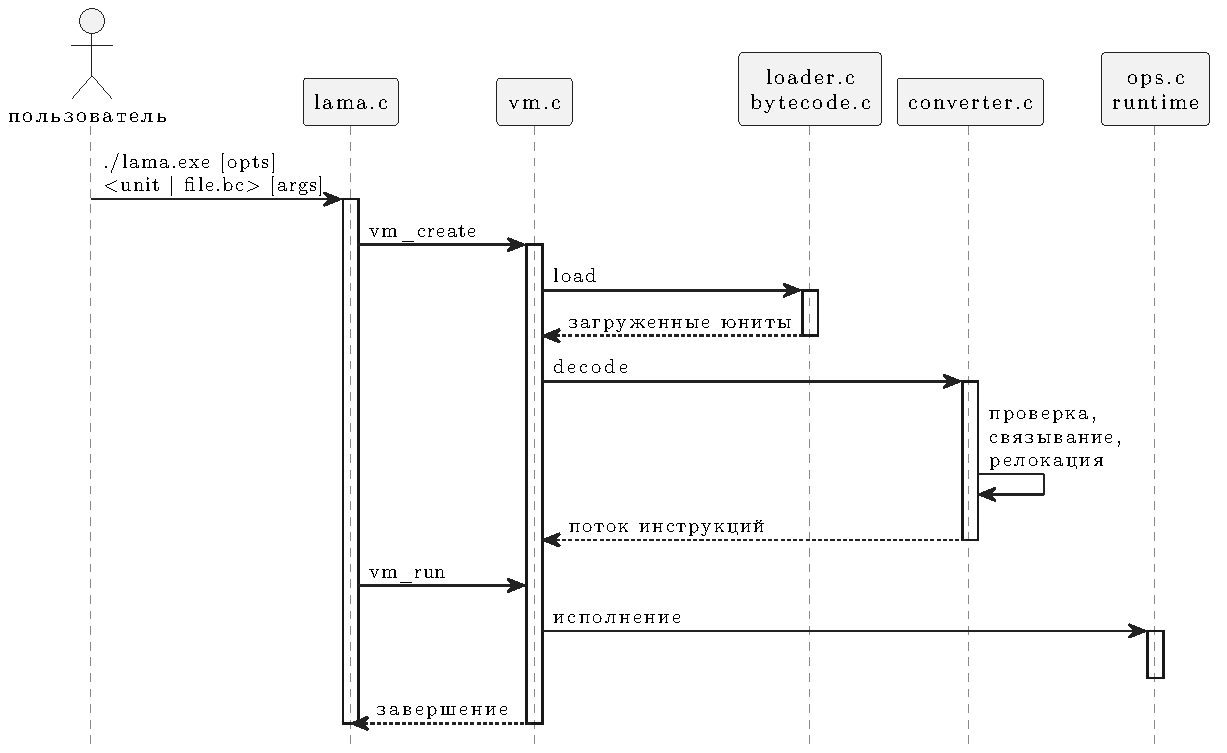
\includegraphics[width=\textwidth]{figures/uml.pdf}
    \caption{Последовательность загрузки, декодирования и исполнения программы.}
    \label{fig:vm-load-run-sequence}
\end{figure}

%TODO: diassembly 

Рисунок~\ref{fig:vm-load-run-sequence} показывает тот же набор компонентов уже
не как структуру, а как порядок работы при одном запуске программы. Вызов функции
\verb=vm_create= относится к фазе подготовки: в нее входят поиск байткодных
файлов, чтение зависимостей, проверка, связывание и построение массива
инструкций. После успешной подготовки управление возвращается в \verb=lama.c=,
который вызывает \verb=vm_run=. На этой фазе \verb=vm.c= инициализирует среду
выполнения, передает аргументы программы и запускает исполнение с первой
инструкции. После возврата из программы виртуальная машина завершает работу
среды выполнения.

Ключевыми архитектурными решениями являются стековая модель исполнения,
предварительная конвертация байткода в массив инструкций и их операндов и явное разделение
загрузки, связывания и исполнения. Стековая модель соответствует байткоду,
порождаемому компилятором Lama. Предварительная конвертация переносит
проверку переходов, ссылок и стековых эффектов в фазу подготовки программы.
